\section*{Profile}
\addcontentsline{toc}{section}{Profile}

\noindent
\begin{tabularx}{\textwidth}{@{} l X @{}}
	\toprule
	Full name   & Muhammad Riduwan Khafidi               \\
	Nickname    & Ridwan                                 \\
	Age         & 18 years old                           \\
	Location    & Batu Aji, Batam, Riau Islands          \\
	Institution & Politeknik Negeri Batam                \\
	Department  & Informatics                            \\
	Study       & Software Engineering Technology (TRPL) \\
	Student ID  & 4342611034                             \\
	Status      & Active student; working while studying \\
	\bottomrule
\end{tabularx}

\section*{Contact \& Repositories}
\addcontentsline{toc}{section}{Contact \& Repositories}

\noindent
\begin{tabularx}{\textwidth}{@{} l X @{}}
	\toprule
	Personal Email & \href{mailto:mroczect@proton.me}{\nolinkurl{mroczect@proton.me}}                                   \\
	Campus Email   & \href{mailto:4342611034@students.polibatam.ac.id}{\nolinkurl{4342611034@students.polibatam.ac.id}} \\
	GitHub         & \href{https://github.com/mroczect}{\nolinkurl{github.com/mroczect}}                                \\
	Codeberg       & \href{https://codeberg.org/mroczect}{\nolinkurl{codeberg.org/mroczect}}                            \\
	\bottomrule
\end{tabularx}

\section*{Papers}
\addcontentsline{toc}{section}{Papers}

\medskip
\noindent\small\textit{The verification table below is automatically generated
	by \texttt{generate\_verification.sh} when \texttt{make all}
	is executed. The file \texttt{content/auto-verification-table.tex}
	must not be edited manually.}

\input{content/auto-verification-table.tex}

\subsection*{Overview}

Every paper in this repository ships with two independent proofs of
integrity stored as sibling files. The two proofs answer different
questions, and neither replaces the other. Both are shown side by
side in Figure~\ref{fig:two-proofs}.

\begin{figure}[H]
	\centering
	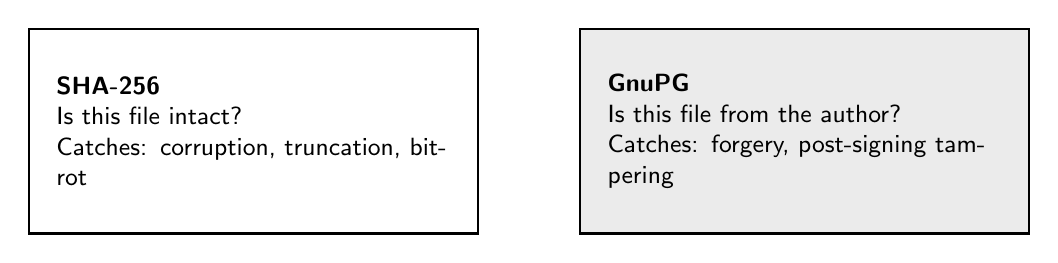
\begin{tikzpicture}[
			box/.style={rectangle, draw=black, thick, text width=5cm,
					minimum height=2.6cm, align=left, font=\sffamily\small,
					inner sep=10pt}
		]
		\node[box, fill=white] (sha) at (-3.5, 0) {
			\textbf{SHA-256} \\
			Is this file intact? \\
			Catches: corruption, truncation, bit-rot
		};
		\node[box, fill=black!8] (gpg) at (3.5, 0) {
			\textbf{GnuPG} \\
			Is this file from the author? \\
			Catches: forgery, post-signing tampering
		};
	\end{tikzpicture}
	\caption{Two independent proofs of integrity, side by side.
		Left: SHA-256 establishes that the file is intact.
		Right: GnuPG establishes that the file is from the author.
		Both must pass before a paper is treated as authentic.}
	\label{fig:two-proofs}
\end{figure}

A SHA-256 checksum alone cannot prove authenticity: anyone who can
modify a file can recompute its checksum. A GnuPG signature alone
cannot rule out corruption: a broken download fails signature
verification for the wrong reason. Together, the two layers
separate three states that would otherwise be indistinguishable:
corrupted in transit, deliberately altered after signing, and
genuine.

The whole procedure takes under a minute for an experienced user
and a few minutes on first try. It requires GnuPG, three essential
commands per paper, and a fingerprint that matches the value
published at the end of Step~1.

\subsection*{The Three Sibling Files}

Each paper has three files sharing the same base name. All three
must be present to complete the verification, as listed in
Table~\ref{tab:sibling-files}.

\begin{table}[H]
	\centering
	\caption{Files shipped alongside each paper.}
	\label{tab:sibling-files}
	\small
	\begin{tabularx}{\textwidth}{@{} l X @{}}
		\toprule
		File                     & Purpose                                                \\
		\midrule
		\texttt{NAME.pdf}        & The document itself, readable by any PDF viewer        \\
		\texttt{NAME.pdf.asc}    & Detached ASCII-armored GnuPG signature                 \\
		\texttt{NAME.pdf.sha256} & One-line SHA-256 checksum in \texttt{sha256sum} format \\
		\bottomrule
	\end{tabularx}
\end{table}

Missing any one of the three breaks the chain. Without the PDF
there is nothing to verify. Without the signature the PDF is
unauthenticated. Without the checksum a corrupted download cannot
be distinguished from a forged one.

\subsection*{Prerequisites}

Install GnuPG on the operating system you will use for
verification. If GnuPG is already installed, skip this section.

\begin{lstlisting}[style=code]
# Debian and Ubuntu
sudo apt install gnupg

# Fedora and RHEL
sudo dnf install gnupg2

# Arch Linux
sudo pacman -S gnupg

# macOS, using Homebrew
brew install gnupg

# Windows, using winget
winget install GnuPG.GnuPG
\end{lstlisting}

Confirm that the binary is available and that the version is 2.2 or
newer:

\begin{lstlisting}[style=code]
gpg --version
\end{lstlisting}

The first line of output names the version. Anything from
\texttt{gpg (GnuPG) 2.2.0} upward works.

\subsection*{Step 1: Import the Author's Public Key}

Every signature in this repository is made with a single RSA key
belonging to the author. The public half of that key ships as
\texttt{public.asc} in the root of this repository, next to this
document.

\begin{lstlisting}[style=code]
gpg --import public.asc
\end{lstlisting}

Expected output, with the key ID shortened here for readability:

\begin{lstlisting}[style=out]
gpg: key B0B3DDCEB6CEF796: public key
     "Muhammad Riduwan Khafidi <mroczect@proton.me>" imported
gpg: Total number processed: 1
gpg:               imported: 1
\end{lstlisting}

The key ID \texttt{B0B3DDCEB6CEF796} is the last sixteen
hexadecimal characters of the full fingerprint. The email address
on the key (\texttt{mroczect@proton.me}) is the author's preferred
address and differs from the institutional address printed on the
title page; both belong to the same person.

\textbf{Importing the key is not the same as trusting it.} A public
key file can be replaced by anyone with write access to the source
it was downloaded from. Before trusting any signature from this
key, verify its fingerprint against an independent channel.

\smallskip
\noindent\textbf{Verify the fingerprint.}
\par\smallskip

\begin{lstlisting}[style=code]
gpg --fingerprint mroczect@proton.me
\end{lstlisting}

Expected output:

\begin{lstlisting}[style=out]
pub   rsa4096 2026-10-01 [SC] [expires: 2028-10-01]
      3D0E 79F1 565A C46E 9EEB  3F49 B0B3 DDCE B6CE F796
uid           [unknown] Muhammad Riduwan Khafidi <mroczect@proton.me>
\end{lstlisting}

The forty-character hexadecimal string on the second line is the
key fingerprint. Compare it, group by group, against the value
below. The spaces in both strings are cosmetic; only the
hexadecimal characters matter.

\par\smallskip
\noindent{\small\texttt{3D0E 79F1 565A C46E 9EEB 3F49 B0B3 DDCE B6CE F796}}
\par\smallskip

This fingerprint is also published on the author's institutional
profile page and on the paper's printed cover. Any of these
channels works as an independent source, provided the channel
itself is not under the author's sole control. If two or more
independent sources agree on the same forty-character value, the
fingerprint is trustworthy.

If the fingerprints match, the key is trustworthy for the purpose
of verifying signatures attributed to this author. If they differ,
stop: the key in \texttt{public.asc} has been replaced and no
further verification should be performed.

The trust line reads \texttt{[unknown]}, which is expected for a
freshly imported key. It means GnuPG has recorded the key but has
not been told that you personally trust it. After you have matched
the fingerprint, you may optionally declare trust so the warning
disappears on subsequent verifications:

\begin{lstlisting}[style=code]
gpg --edit-key mroczect@proton.me trust
# choose 5 (ultimate), then save
\end{lstlisting}

The trust level is a local annotation, not a cryptographic claim.
The cryptographic verification result is identical whether you set
it or not; only the printed warning changes.

\subsection*{Step 2: Download the Three Files}

For each paper you want to verify, download all three sibling files
into the same directory. File names must match exactly, including
the \texttt{.pdf}, \texttt{.asc}, and \texttt{.sha256} suffixes.

\subsection*{Step 3: Verify the SHA-256 Checksum}

The checksum confirms that the downloaded file matches the file
that was signed. A mismatch means either the download was corrupted
or the file was altered after publication.

\begin{lstlisting}[style=code]
# Linux
sha256sum -c NAME.pdf.sha256

# macOS
shasum -a 256 -c NAME.pdf.sha256

# Windows, PowerShell (native)
(Get-FileHash NAME.pdf -Algorithm SHA256).Hash.ToLower() -eq \
  (Get-Content NAME.pdf.sha256 | ForEach-Object { ($_ -split ' ')[0] })

# Windows, cmd (manual comparison)
certutil -hashfile NAME.pdf SHA256
# then compare the output with the line in NAME.pdf.sha256
\end{lstlisting}

On Linux and macOS, the tool compares the values automatically and
prints one of two lines.

Success:

\begin{lstlisting}[style=out]
NAME.pdf: OK
\end{lstlisting}

Failure:

\begin{lstlisting}[style=out]
NAME.pdf: FAILED
sha256sum: WARNING: 1 computed checksum did NOT match
\end{lstlisting}

On Windows, the PowerShell one-liner above compares the two values
automatically and prints \texttt{True} or \texttt{False}.
\texttt{certutil} requires manual comparison; both strings are
sixty-four hexadecimal characters.

A \texttt{FAILED} result means the file is unusable. Do not open
the PDF. Delete it, download again, and repeat this step. If the
second download also fails, the copy on the server has been
modified and the author should be contacted.

\subsection*{Step 4: Verify the GnuPG Signature}

The signature confirms that the file was signed by the holder of
the author's private key, and that the file has not been modified
since the signature was made.

\begin{lstlisting}[style=code]
gpg --verify NAME.pdf.asc NAME.pdf
\end{lstlisting}

Expected output for a key whose fingerprint has been verified but
whose trust level has not been declared:

\begin{lstlisting}[style=out]
gpg: Signature made Sun Nov  2 23:10:00 2026 WIB
gpg:                using RSA key 3D0E79F1565AC46E9EEB3F49B0B3DDCEB6CEF796
gpg: Good signature from "Muhammad Riduwan Khafidi <mroczect@proton.me>" [unknown]
gpg: WARNING: This key is not certified with a trusted signature!
gpg:          There is no indication that the signature belongs to the owner.
Primary key fingerprint: 3D0E 79F1 565A C46E 9EEB  3F49 B0B3 DDCE B6CE F796
\end{lstlisting}

Read the output line by line.

The first line gives the signature creation date, in the signer's
local timezone. This date is covered by the signature and cannot
be forged without invalidating the entire signature.

The second line gives the key fingerprint without spaces, which
must match the spaced fingerprint verified in Step~1. Only the
hexadecimal characters matter.

The third line reads \texttt{Good signature from} followed by the
signer's name and email. This is the cryptographic confirmation
that the PDF matches the signed content byte for byte.

The warning about the uncertified key is expected. It disappears
only after you have declared your trust with the command shown at
the end of Step~1. The warning does not mean the signature is
invalid; it means you have not yet told GnuPG that you trust the
key itself. If you have verified the fingerprint manually, the
warning can be ignored.

The final line repeats the fingerprint so you do not need to
scroll up to Step~1 to compare.

\subsection*{Step 5: Read the Signature Timestamp}

The signature creation date is the third fact that cryptographic
verification establishes. It confirms that the signature was made
when the author said it was made, and it tells you which version
of the paper you are looking at.

The timestamp is stored inside the \texttt{.asc} file as a Unix
epoch value. To read it:

\begin{lstlisting}[style=code]
gpg --list-packets NAME.pdf.asc | grep created
\end{lstlisting}

The output includes a line of the form \texttt{created <number>}.
The number is seconds since 1970. To convert it to a human-readable
date on Linux:

\begin{lstlisting}[style=code]
ts=$(gpg --list-packets NAME.pdf.asc | \
     sed -n 's/.*created *\([0-9]*\).*/\1/p' | head -n 1)
date -d "@$ts" +"%Y-%m-%d %H:%M:%S %Z"
\end{lstlisting}

On macOS, replace the last line with:

\begin{lstlisting}[style=code]
date -r "$ts"
\end{lstlisting}

If the date you obtain here differs from the date printed by
\texttt{gpg --verify} in Step~4, trust the \texttt{gpg --verify}
output. The signature carries the timestamp; the displayed date is
derived directly from it. A mismatch between this date and any
external document (such as a printed cover) may simply mean the
document was updated after the signature was made, but the
signature itself remains authoritative for the version it signed.

\subsection*{Troubleshooting}

\begin{table}[H]
	\centering
	\caption{Failure modes and their meaning.}
	\label{tab:troubleshooting}
	\footnotesize
	\begin{tabularx}{\textwidth}{>{\raggedright\arraybackslash}p{4.2cm} X X}
		\toprule
		Message                                       & Cause                                                                               & Remedy                                                                                 \\
		\midrule
		\texttt{BAD signature}                        & The PDF differs from the file that was signed; strongest possible warning           & Do not open the PDF. Delete all three files and re-download from the source            \\
		\texttt{Can't check signature: No public key} & The author's public key is not in this keyring                                      & Repeat Step 1                                                                          \\
		\texttt{Good signature ... [unknown]}         & Signature is cryptographically valid, but the key has not been declared trustworthy & Verify the fingerprint per Step 1, then optionally mark the key as trusted             \\
		\texttt{Good signature ... [expired]}         & The key that made the signature has passed its expiration date                      & Check the fingerprint per Step 1. Contact the author for an updated key if needed      \\
		\texttt{Good signature ... [revoked]}         & The key has been revoked by its owner; signature must not be trusted                & Contact the author through a channel other than email. Do not use the file             \\
		\texttt{sha256sum: FAILED}                    & The computed checksum differs from the recorded one                                 & Re-download. If the failure persists, the file on the server has been altered          \\
		\texttt{gpg: no valid OpenPGP data found}     & The \texttt{.asc} file is corrupt, empty, or not an armored signature               & Re-download. Confirm the file begins with the line shown in the note below             \\
		\texttt{gpg: CRC error}                       & The armored signature was truncated or corrupted in transit                         & Re-download \texttt{NAME.pdf.asc}                                                      \\
		\texttt{No such file or directory}            & The three files are in different directories, or a filename has a typo              & Move all three files into the same directory. Confirm exact filenames with \texttt{ls} \\
		\bottomrule
	\end{tabularx}
\end{table}

\par\smallskip
\noindent The first line of a valid armored signature is
	{\small\texttt{\detokenize{-----BEGIN PGP SIGNATURE-----}}}.
\par\smallskip

The most important line in the failure table is the first.
\texttt{BAD signature} means the PDF on your disk is not the PDF
the author signed. Whether the difference came from a network
attack or a corrupted write, the file cannot be trusted.

The second most important line is \texttt{[unknown]}. Most readers
see this on their first verification and assume the check failed.
It did not. The signature is valid; the warning is a separate
question about whether you personally have decided the key belongs
to the author. Step~1 is how you answer that question.

\subsection*{Batch Verification}

To verify every paper in a directory at once, assuming the papers
live in \texttt{paper/} and that every paper has its matching
\texttt{.asc} and \texttt{.sha256} siblings:

\begin{lstlisting}[style=code]
for asc in paper/*.pdf.asc; do
    pdf="${asc%.asc}"
    sha="${pdf}.sha256"
    echo "== $(basename "$pdf") =="
    sha256sum -c "$sha" 2>&1 | grep -E 'OK|FAILED'
    gpg --verify "$asc" "$pdf" 2>&1 \
        | grep -E 'Good|BAD|Can.t|no valid|CRC'
done
\end{lstlisting}

The \texttt{sha256sum} check runs first. If it fails, delete the
file and re-download before running the signature check. The
\texttt{grep} filters keep only the lines that matter: success
(\texttt{OK}, \texttt{Good signature}) and every failure mode that
warrants attention (\texttt{FAILED}, \texttt{BAD}, \texttt{Can't
	check}, \texttt{no valid}, \texttt{CRC}). For a single paper, use
the full command from Step~4.

\subsection*{Quick Reference}

\begin{table}[H]
	\centering
	\caption{Every command in this guide.}
	\label{tab:quick-reference}
	\footnotesize
	\begin{tabularx}{\textwidth}{l X}
		\toprule
		Purpose                           & Command                                                   \\
		\midrule
		Install GnuPG on Debian or Ubuntu & \texttt{sudo apt install gnupg}                           \\
		Install GnuPG on macOS            & \texttt{brew install gnupg}                               \\
		Import the author's public key    & \texttt{gpg -{}-import public.asc}                        \\
		Print the key fingerprint         & \texttt{gpg -{}-fingerprint mroczect@proton.me}           \\
		Mark the key as trusted           & \texttt{gpg -{}-edit-key mroczect@proton.me trust}        \\
		Verify SHA-256 on Linux           & \texttt{sha256sum -c NAME.pdf.sha256}                     \\
		Verify SHA-256 on macOS           & \texttt{shasum -a 256 -c NAME.pdf.sha256}                 \\
		Verify SHA-256 on PowerShell      & \texttt{(Get-FileHash NAME.pdf -Algorithm SHA256).Hash}   \\
		Verify the GnuPG signature        & \texttt{gpg -{}-verify NAME.pdf.asc NAME.pdf}             \\
		Read the signature creation date  & \texttt{gpg -{}-list-packets NAME.pdf.asc | grep created} \\
		Verify every paper in one pass    & loop shown in the Batch Verification section              \\
		\bottomrule
	\end{tabularx}
\end{table}

The whole procedure fits in a single sentence: import the key,
verify its fingerprint against an independent source, then run
\texttt{gpg -{}-verify} on each paper. Everything else in this
guide exists to explain why each of those three steps matters and
what can go wrong at each one.


\medskip
\noindent\rule{\textwidth}{0.4pt}
\medskip

\noindent\textit{Note: this document is created for administrative
	purposes and self-introduction. The author is not yet proficient in
	programming and does not claim otherwise.}
